\newpage
\section{The Processor}
\begin{figure}[!htb]
    \centering
    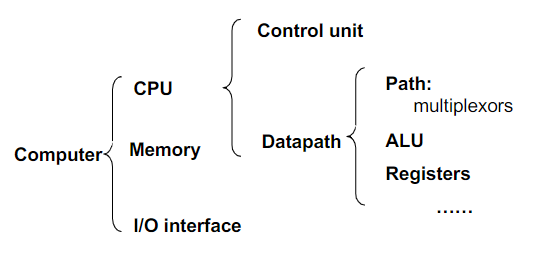
\includegraphics[width=0.199\textwidth]{CO4/Comptuer Organization}
    \caption{Comptuer Organization}
\end{figure}

\subsection{Introduction}
\begin{itemize}
    \item CPU performance factors
    \begin{itemize}
        \item\small Instruction count: Determined by ISA and compiler
        \item\small CPI and Cycle time: Determined by CPU hardware
    \end{itemize}
    \item implementations
    \begin{itemize}
        \item\small A simplified version
        \item\small A more realistic pipelined version
    \end{itemize}
    \item Simple subset, shows most aspects
\end{itemize}

\subsubsection{An overview of Implementation}

\begin{figure}[!htb]
    \centering
    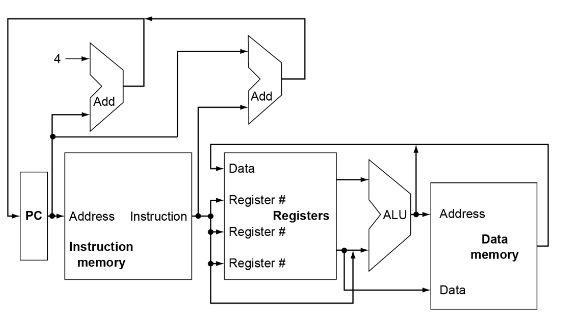
\includegraphics[width=0.309\textwidth]{CO4/An overview of Implementation}
    \caption{An overview of Implementation}
\end{figure}

Must use multiplexers to join wires together. 

\subsubsection{Control}
Control the units: Read Memory, Write Memory. (blue wires are control)

\begin{figure}[!htb]
    \centering
    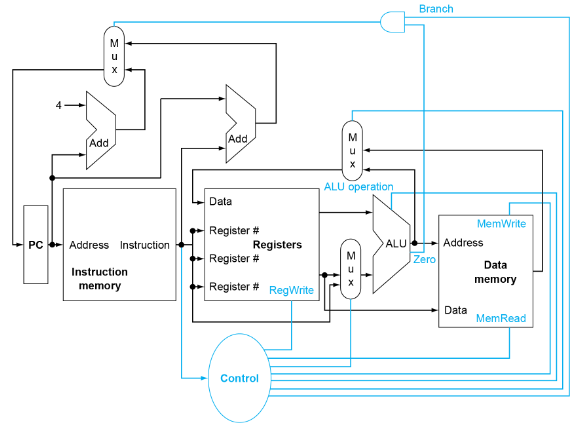
\includegraphics[width=0.309\textwidth]{CO4/Control}
    \caption{Control}
\end{figure}

\subsection{Logic Design Conventions}
\begin{itemize}
    \item Combinational element
    \begin{itemize}
        \item\small Operate on data
        \item\small Output is a function of input
    \end{itemize}
    \item State (sequential) elements: \small Store information
\end{itemize}

% \subsubsection{Combinational Elements}

% \subsubsection{State (sequential) elements}

\subsubsection{Clocking Methodology}
Combinational logic transforms data during clock cycles. 

\begin{figure}[!htb]
    \centering
    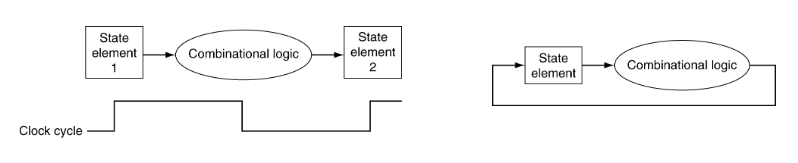
\includegraphics[width=0.479\textwidth]{CO4/Clocking Methodology}
    \caption{Clocking Methodology}
\end{figure}

\subsection{Building a Datapath}
Datapath is elements that process data and addresses in the CPU. 

\subsubsection{Instruction execution in RISC-V}
\begin{enumerate}
    \item Fetch :
    \begin{enumerate}
        \item\small Take instructions from the instruction memory
        \item\small Modify PC to point the next instruction
    \end{enumerate}
    \item Instruction decoding \& Read Operand:
    \begin{enumerate}
        \item\small Will be translated into machine control command
        \item\small Reading Register Operands, whether or not to use
        \item\small Reading Register Operands, whether or not to use
    \end{enumerate}
    \item Executive Control:
    \begin{enumerate}
        \item\small Control the implementation of the corresponding ALU operation
    \end{enumerate}
    \item Memory access:
    \begin{enumerate}
        \item\small Write or Read data from memory
        \item\small Only ld/sd
    \end{enumerate}
    \item Write results to register:
    \begin{enumerate}
        \item\small If it is R-type instructions, ALU results are written to rd
        \item\small If it is I-type instructions, memory data are written to rd
    \end{enumerate}
\end{enumerate}
\begin{itemize}
    \item Modify PC for branch instructions: \small Can be everywhere
\end{itemize}

\subsubsection{Instruction Fetch}
\begin{figure}[!htb]
    \centering
    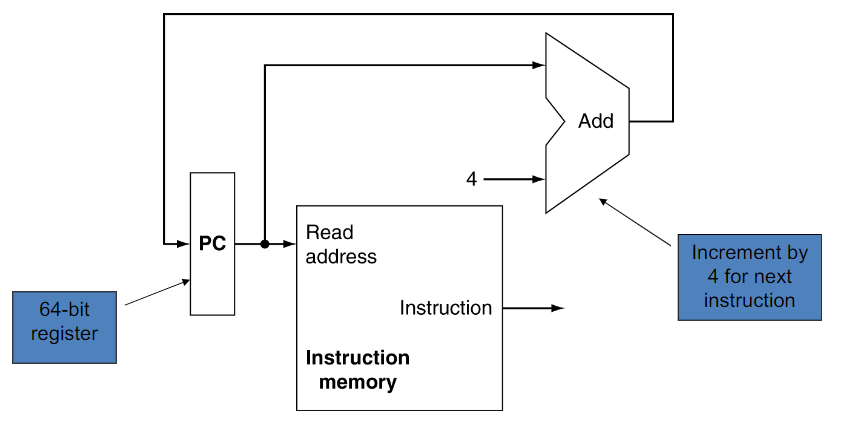
\includegraphics[width=0.309\textwidth]{CO4/Instruction Fetch}
    \caption{Instruction Fetch}
    \label{Instruction Fetch}
\end{figure}
[\ref{Instruction Fetch}]


\subsubsection{R-Format Instructions}
\begin{enumerate}
    \item Read two register operands
    \item Perform arithmetic/logical operation
    \item Write register result
\end{enumerate}

\begin{figure}[!htb]
    \centering
    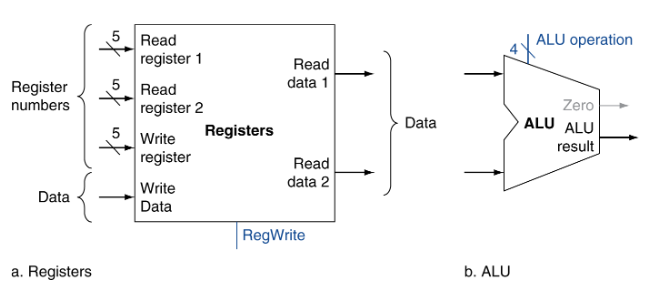
\includegraphics[width=0.309\textwidth]{CO4/R-Format Instructions}
    \caption{R-Format Instructions}
\end{figure}

\subsubsection{Load/Store Instructions}
\begin{enumerate}
    \item Read register operands
    \item Calculate address using 12-bit offset 
    
    \small Use ALU, but sign-extend offset
    \item Load: Read memory and update register
    \item Store: Write register value to memory
\end{enumerate}

\begin{figure}[!htb]
    \centering
    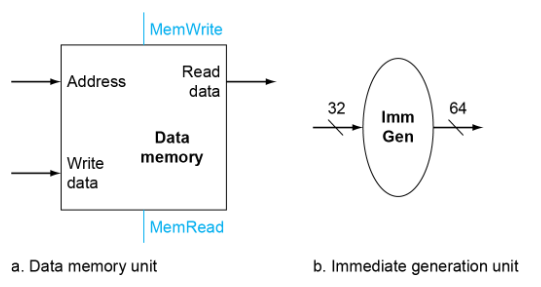
\includegraphics[width=0.309\textwidth]{CO4/Load Store Instructions}
    \caption{Load/Store Instructions}
\end{figure}

\subsubsection{Branch Instructions}
\begin{enumerate}
    \item Read register operands
    \item Compare operands 
    
    \small Use ALU, subtract and check Zero output
    \item Calculate target address
    \begin{enumerate}
        \item\small Sign-extend displacement
        \item\small Shift left 1 place (halfword displacement)
        \item\small Add to PC value
    \end{enumerate}
\end{enumerate}

\begin{figure}[!htb]
    \centering
    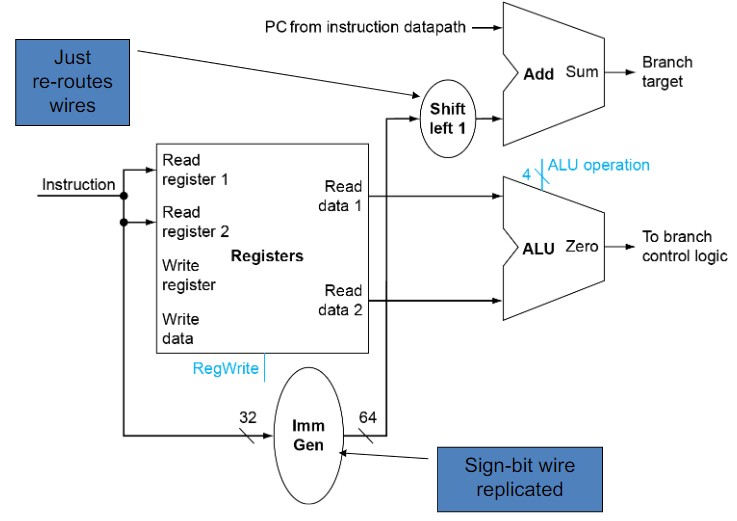
\includegraphics[width=0.309\textwidth]{CO4/Branch Instructions}
    \caption{Branch Instructions}
\end{figure}

\subsubsection{Composing the Elements}
\begin{enumerate}
    \item First-cut data path does an instruction in one clock cycle. Each datapath element can only do one function at a time. Hence, we need separate instruction and data memories. 
    \item Use multiplexers where alternate data sources are used for different instructions
\end{enumerate}

\subsubsection{Path Built using Multiplexer}
\begin{itemize}
    \item R-type instruction Datapath
    \item I-type instruction Datapath
    \begin{itemize}
        \item\small For ALU
        \item\small For load
    \end{itemize}
    \item S-type (store) instruction Datapath
    \item SB-type (branch) instruction Datapath
    \item UJ-type instruction Datapath
    \begin{itemize}
        \item\small  For Jump
    \end{itemize}
\end{itemize}

\begin{enumerate}
    \item R type Instruction \& Data stream
    \item I type Instruction \& Data stream
    
    (下方 Sign extend 可以直接为 imm Gen)
    \item S type Instruction \& Data stream
    \item SB type Instruction \& Data stream
    
    (最右上角PC from instruction datapath 不过add的需要 PC+4)
    \item Jal/J type Instruction \& Data stream
    
    (这个图不太对)
\end{enumerate}
%UNTODO add fig P30-P35

\subsubsection{Full Datapath}
\begin{figure}[!htb]
    \centering
    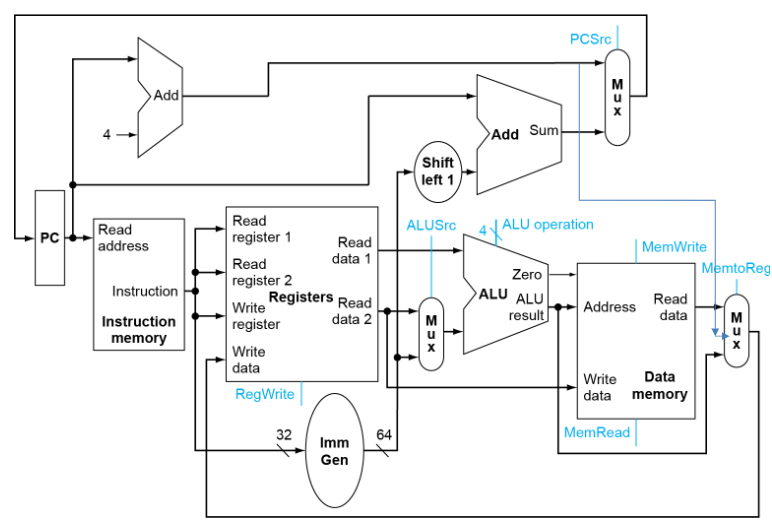
\includegraphics[width=0.47\textwidth]{CO4/Full Datapath}
    \caption{Full Datapath}
    \label{Full Datapath}
\end{figure}
\ref{Full Datapath}

\subsection{A Simple Implementation Scheme}
\subsubsection{Building Controller}
There are 7+4 signals

\begin{figure}[!htb]
    \centering
    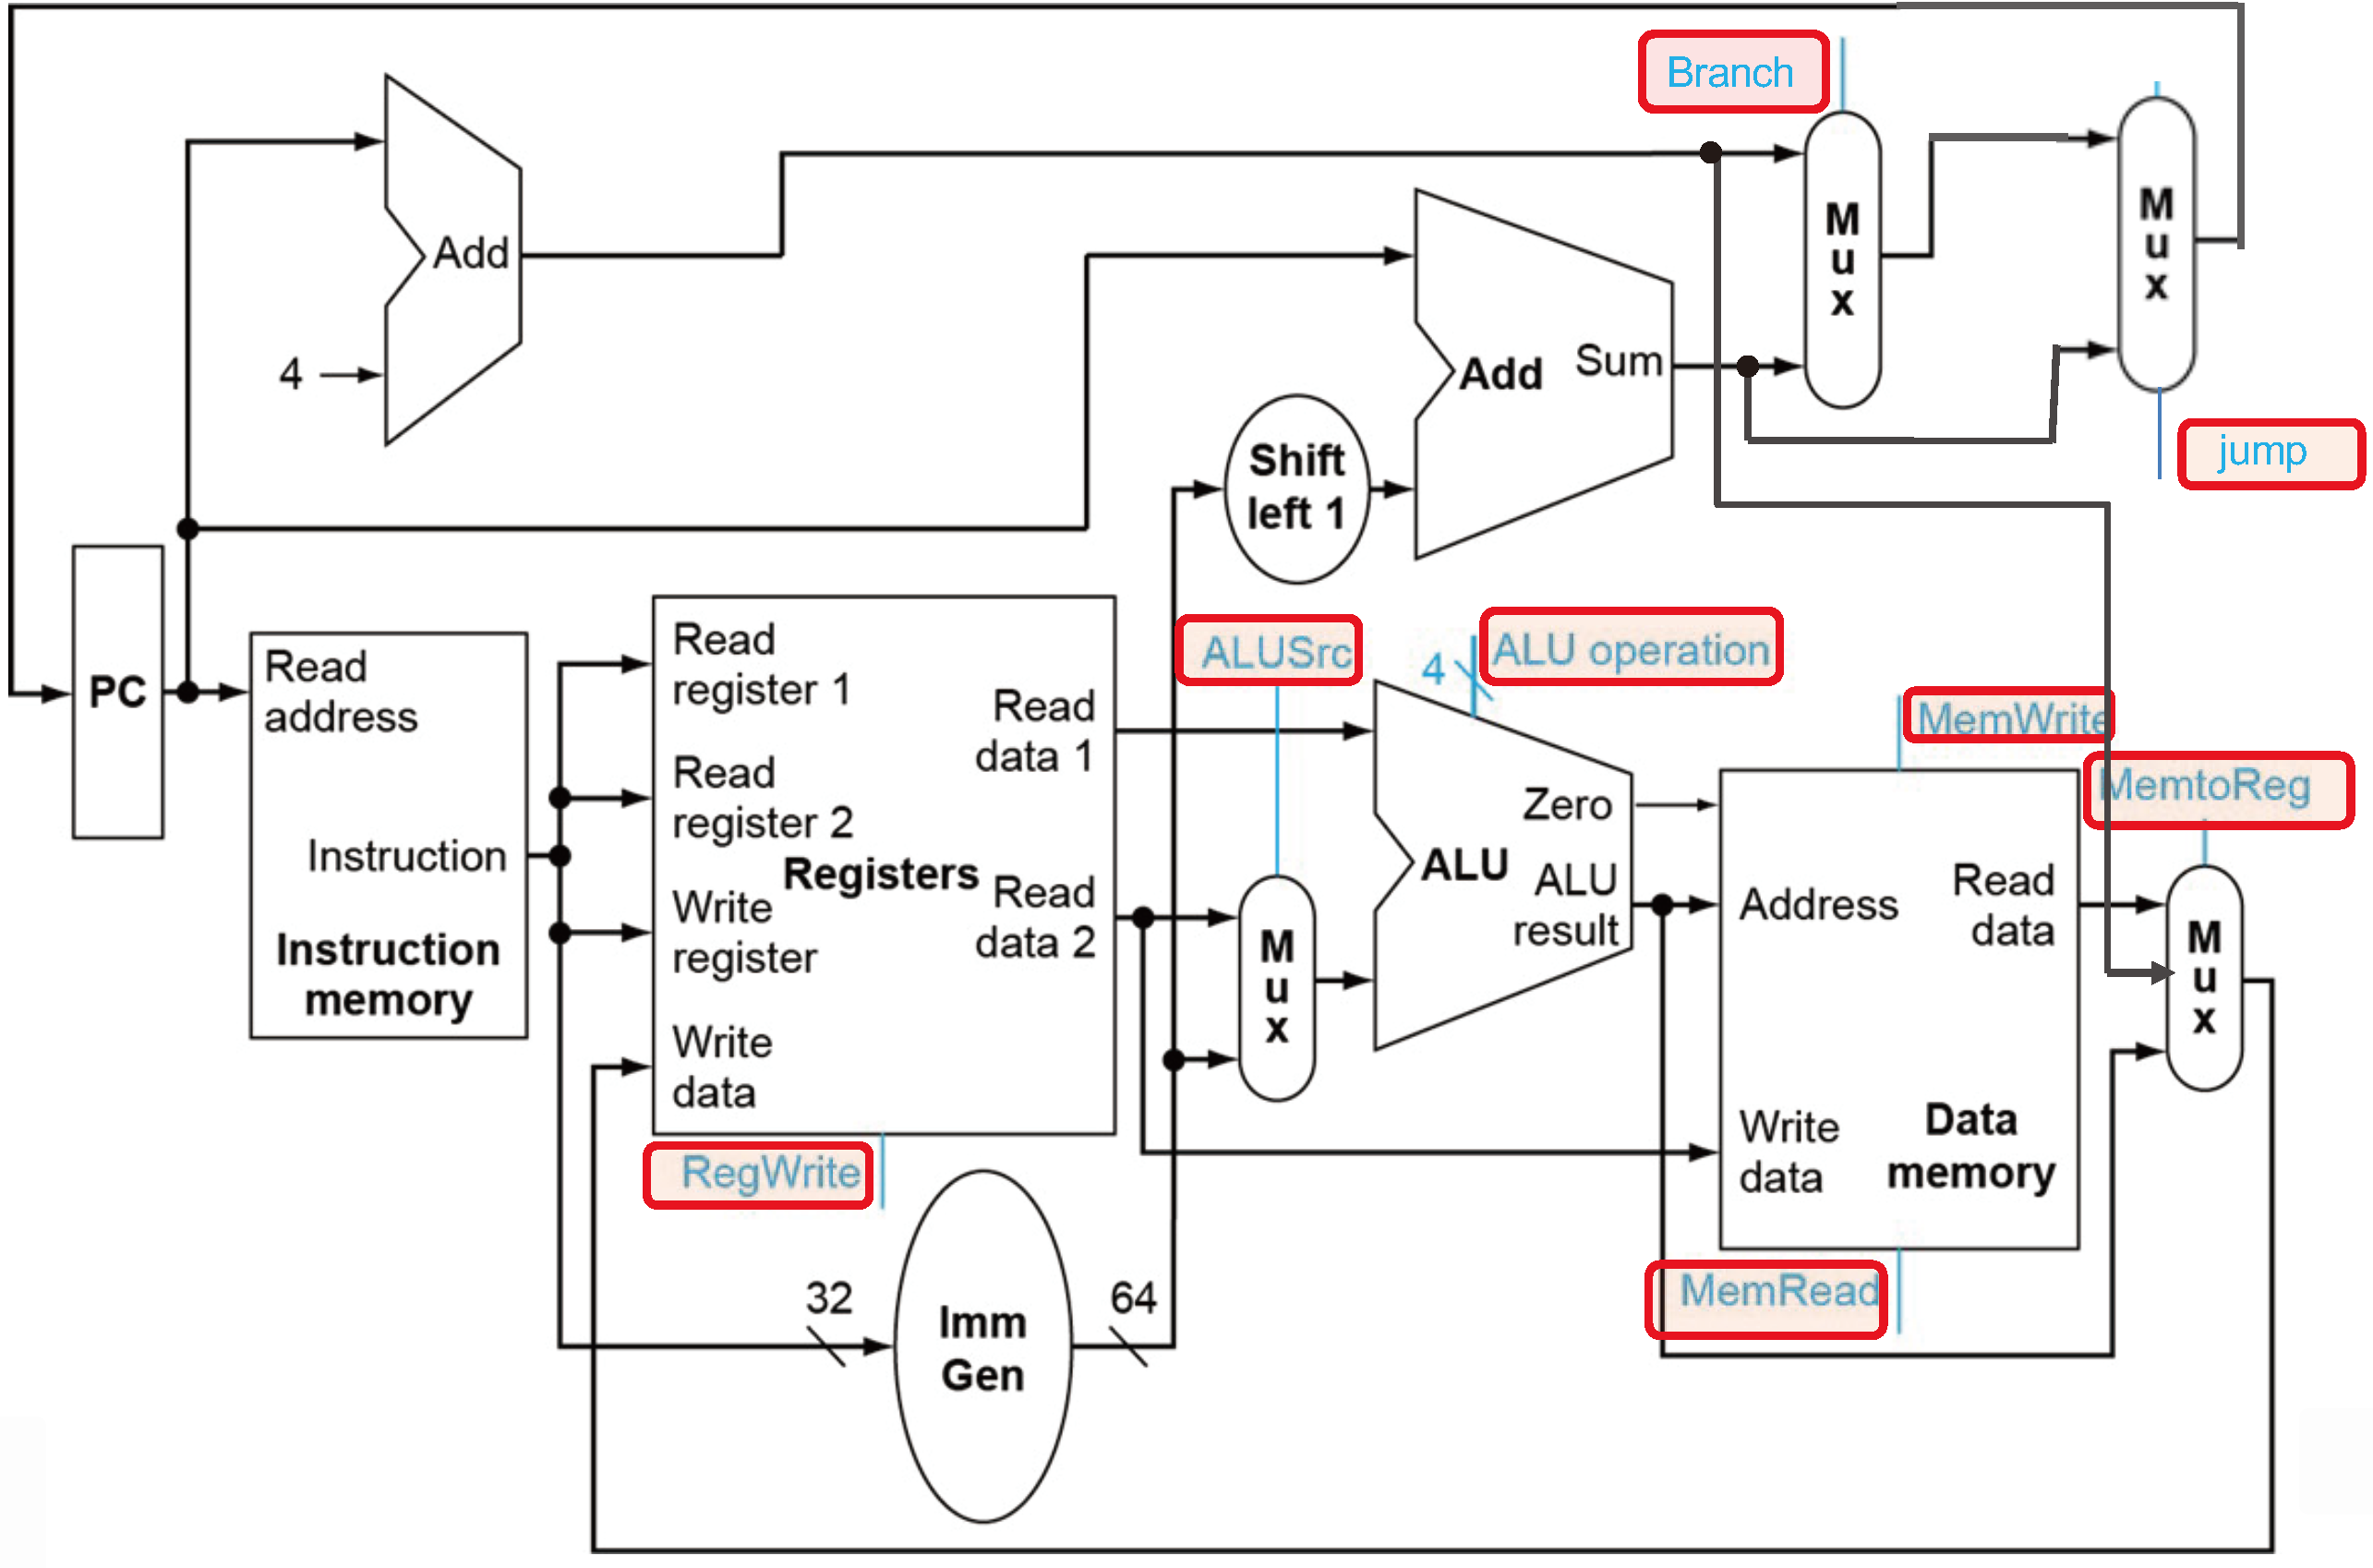
\includegraphics[width=0.47\textwidth]{CO4/Building Controller}
    \caption{Building Controller}
\end{figure}

\subsubsection{Scheme of Controller}
\begin{figure}[!htb]
    \centering
    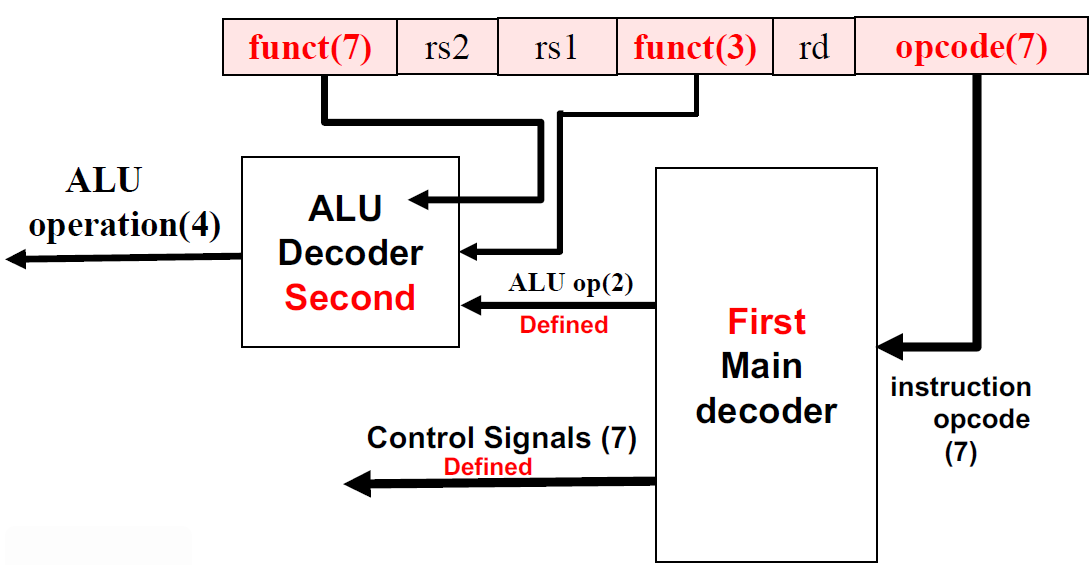
\includegraphics[width=0.309\textwidth]{CO4/Scheme of Controller}
    \caption{Scheme of Controller}
    \label{Scheme of Controller}
\end{figure}
\ref{Scheme of Controller}

\subsubsection{Designing the Main Control Unit --- First level}

% \subsubsection{Truth tables \& Circuitry of main Controller}
Main Control Unit function
\begin{enumerate}
    \item ALU op (2)
    \item Divided 7 control signals into 2 groups
    \begin{itemize}
        \item\small 4 Mux
        \item\small 3 R/W
    \end{itemize}
\end{enumerate}

\begin{figure}[!htb]
    \centering
    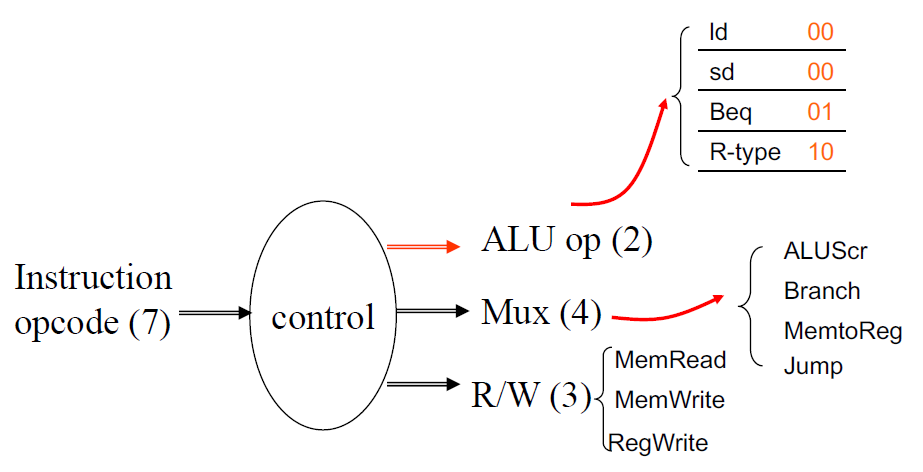
\includegraphics[width=0.309\textwidth]{CO4/Main Control Unit}
    \caption{Main Control Unit}
\end{figure}

\begin{table}[!htb]
    \centering
    \caption{Truth tables of main Controller}
    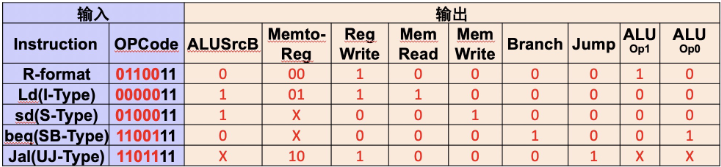
\includegraphics[width=0.479\textwidth]{CO4/Truth tables of main Controller}
\end{table}

\subsubsection{Design the ALU Decoder second level}
ALU used for
\begin{enumerate}
    \item\small Load/Store: F = add
    \item\small Branch: F = subtract
    \item\small R-type: F depends on opcode
\end{enumerate}

\begin{table}[!htb]
    \centering
    \caption{ALU Decoder}
    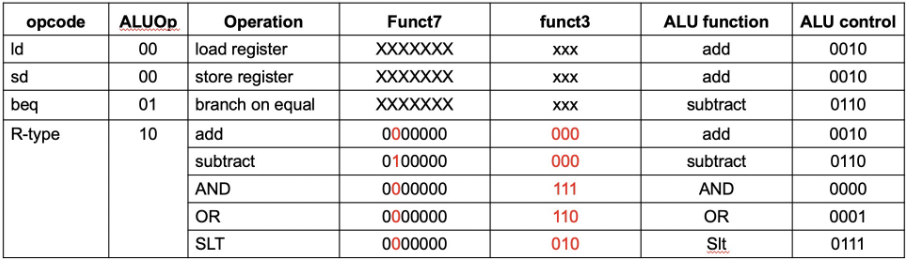
\includegraphics[width=0.479\textwidth]{CO4/ALU Decoder}
\end{table}


\subsubsection{Datapath with Control}
\ref{Datapath with Control}
\begin{figure}[!htb]
    \centering
    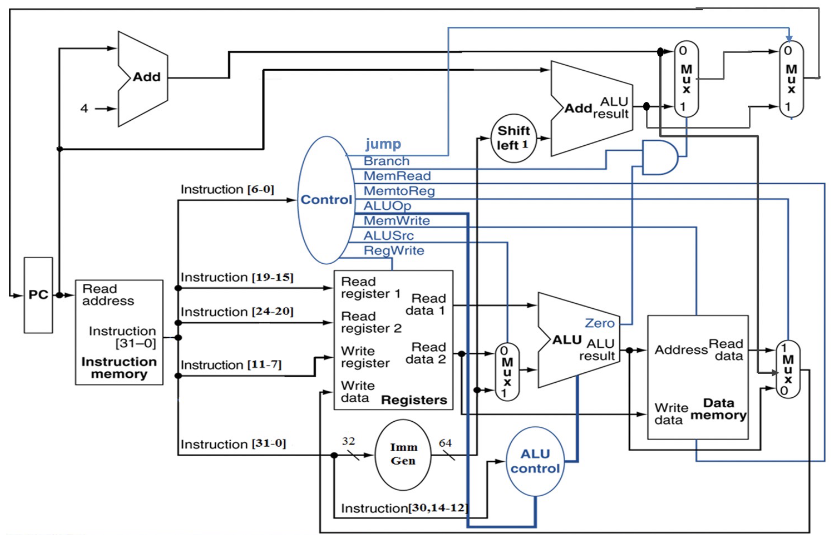
\includegraphics[width=0.479\textwidth]{CO4/Datapath with Control}
    \caption{Datapath with Control}
    \label{Datapath with Control}
\end{figure}

\subsection{An overview of pipelining}

\subsubsection{Performance Issues}
Longest delay of Critical path (load instruction) determines clock period. Wihout violating design principle: Making the common case fast, we will improve performance by pipelining

\paragraph{Pipelining Analogy}
Pipelined laundry: overlapping execution

\subsubsection{RISC-V Pipeline}
Five stages:
\begin{enumerate}\small
    \item IF: Instruction fetch from memory
    \item ID: Instruction decode \& register read
    \item EX: Execute operation or calculate address
    \item MEM: Access memory operand
    \item WB: Write result back to register    
\end{enumerate}

\paragraph{Pipelining RISC-V instruction set}
CPI is decreased to 1, since one instruction will be issued (or finished) each cycle. 

During any cycle, one instruction is present in each stage.

\begin{figure}[!htb]
    \centering
    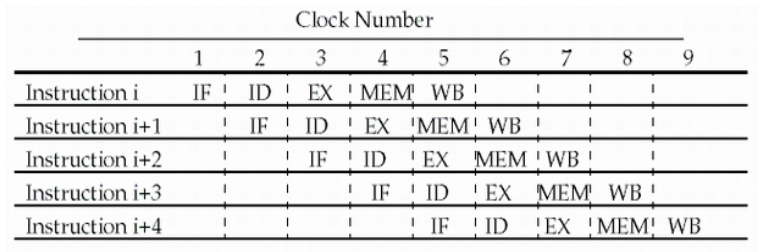
\includegraphics[width=0.42\textwidth]{CO4/Pipelining RISC-V instruction set}
    \caption{Pipelining RISC-V instruction set}
\end{figure}

Ideally, performance is increased five fold!

\paragraph{Pipeline Performance}
\begin{figure}[!htb]   
    \centering
    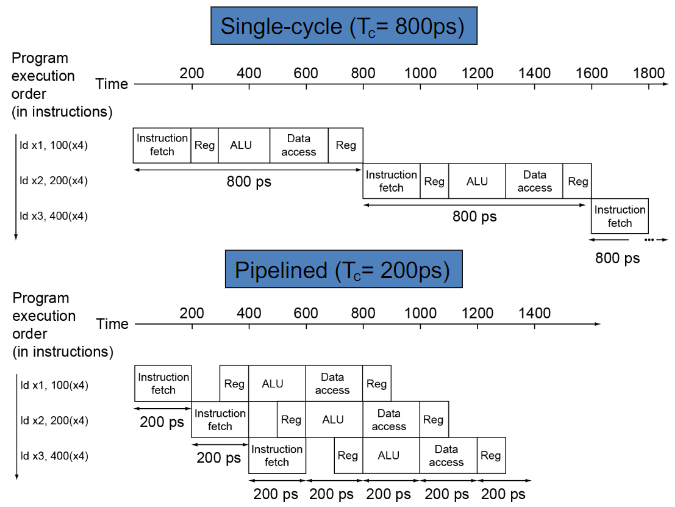
\includegraphics[width=0.329\textwidth]{CO4/Pipeline Performance}
    \caption{Pipeline Performance}
\end{figure}

Reg滞后是防止读写冲突. 

\paragraph{Pipeline Speedup}
If all stages are balanced, i.e., all take the same time. 
\begin{align*}
    &\text{Time between instructions}_{\text{pipelined}}\\
    =&\frac{\text{Time between instruction}_{\text{pipelined}}}{\text{Number of stages}}
\end{align*}

If not balanced, speedup is less. 

Speedup due to increased throughput
n Latency (time for each instruction) does not
decrease

\paragraph{Pipelining and ISA Design}
RISC-V ISA designed for pipelining

\begin{enumerate}\small
    \item All instructions are 32-bits
    \subitem Easier to fetch and decode in one cycle
    \subitem c.f. x86: 1- to 17-byte instructions
    \item Few and regular instruction formats
    \subitem Can decode and read registers in one step
    \item Load/store addressing
    \subitem Can calculate address in 3rd stage, access memory in 4th stage
\end{enumerate}

\subsubsection{Hazards}

Situations that prevent starting the next instruction in the next cycle. 

\begin{enumerate}
    \item \textbf{Structure hazards}: A required resource is busy
    \item \textbf{Data hazard}: Need to wait for previous instruction to complete its data read/write
    \item \textbf{Control hazard}: Deciding on control action depends on previous instruction
\end{enumerate}

\subsubsection{Structure Hazards}
Conflict for use of a resource. 

In RISC-V pipeline with a single memory, Load/store requires data access but instruction fetch would have to stall for that cycle which would cause a pipeline ``bubble''. 

Hence, pipelined datapaths require separate instruction/data memories, or separate instruction/data caches. 

\subsubsection{Data Hazard}
An instruction depends on completion of data access by a previous instruction. 

\begin{lstlisting}[language={[x86masm]Assembler}]
add x19, x0, x1
sub x2, x19, x3
\end{lstlisting}

\begin{figure}[!htb]
    \centering
    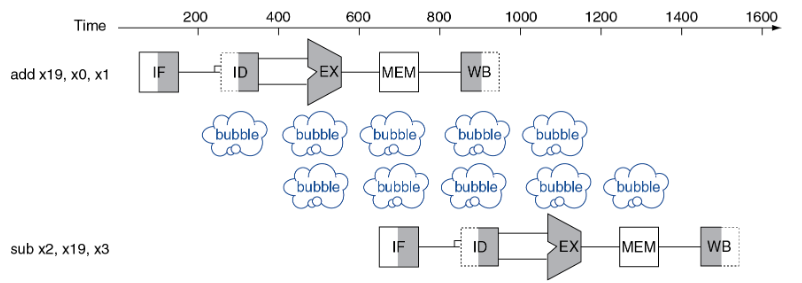
\includegraphics[width=0.309\textwidth]{CO4/Data Hazard}
    \caption{Data Hazard}
\end{figure}

\paragraph{Forwarding (aka Bypassing)}
Use result when it is computed. Don't wait for it to be stored in a register. But requires extra connections in the datapath. 

\begin{figure}[!htb]
    \centering
    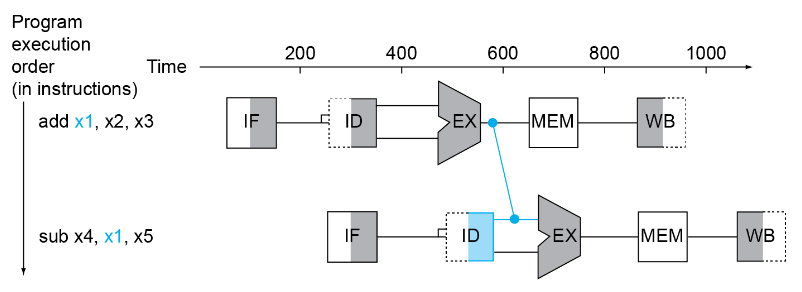
\includegraphics[width=0.309\textwidth]{CO4/Forwarding}
    \caption{Forwarding}
\end{figure}

\paragraph{Load-Use Data Hazard}

Can't always avoid stalls by forwarding. If value not computed when needed, can't forward backward in time!

\begin{figure}[!htb]
    \centering
    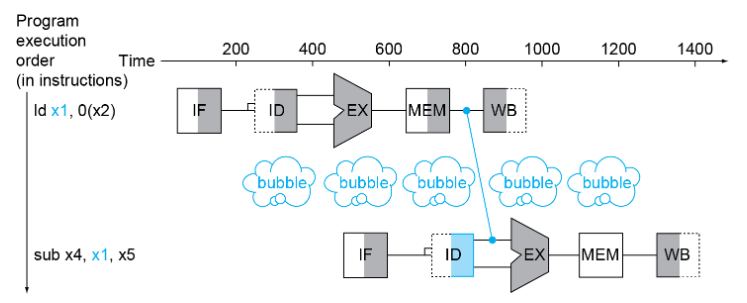
\includegraphics[width=0.309\textwidth]{CO4/Load-Use Data Hazard}
    \caption{Load-Use Data Hazard}
\end{figure}

\paragraph{Code Scheduling to Avoid Stalls}
Reorder code to avoid use of load result in the next instruction. 

\begin{lstlisting}[language={C}]
a=b+e;
c=b+f;
\end{lstlisting}

\begin{figure}[!htb]
    \centering
    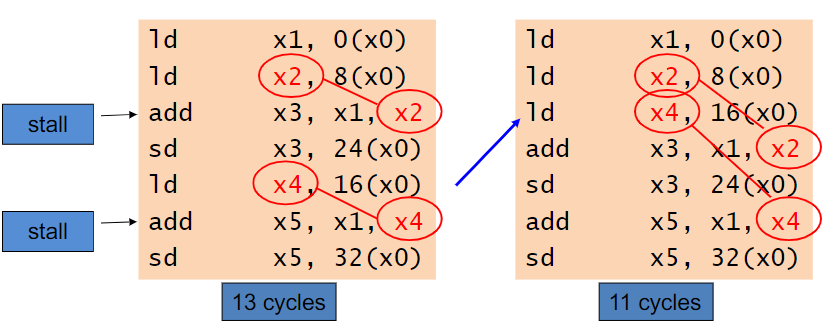
\includegraphics[width=0.309\textwidth]{CO4/Code Scheduling to Avoid Stalls}
    \caption{Code Scheduling to Avoid Stalls}
\end{figure}

\subsubsection{Control Hazards}
Branch determines flow of control. Fetching next instruction depends on branch outcome. Pipeline can't always fetch correct instruction, Still working on ID stage of branch. 

In RISC-V pipeline, need to compare registers and compute target early in the pipeline, add hardware to do it in ID stage.

\paragraph{Stall on Branch}
Wait until branch outcome determined before fetching next instruction. 
\begin{figure}[!htb]
    \centering
    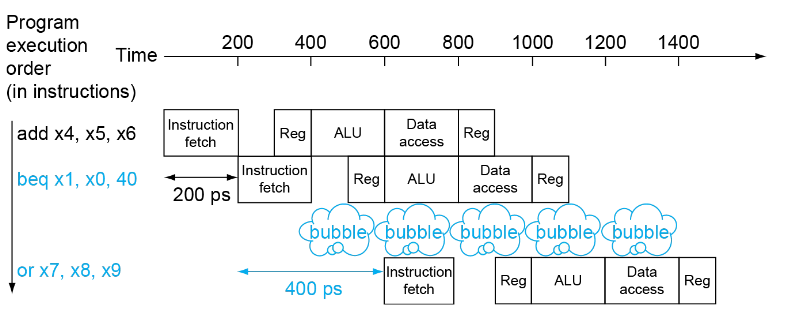
\includegraphics[width=0.309\textwidth]{CO4/Stall on Branch}
    \caption{Stall on Branch}
\end{figure}

\paragraph{Branch Prediction}
Longer pipelines can't readily determine branch outcome early. Can predict outcome of branch, only stall if prediction is wrong. 

In RISC-V pipeline, Can predict branches not taken and Fetch instruction after branch, with no delay

\paragraph{More-Realistic Branch Prediction}
\begin{itemize}
    \item \textbf{Static branch prediction}: Based on typical branch behavior
    \item \textbf{Dynamic branch prediction}: Hardware measures actual branch behavior, assume future behavior will continue the trend. 
\end{itemize}

\subsubsection{Pipeline Summary}
Pipelining improves performance by increasing instruction throughput. 
\begin{itemize}
    \item Executes multiple instructions in parallel
    \item Each instruction has the same latency
\end{itemize}
Subject to hazards: Structure, data, control

Instruction set design affects complexity of pipeline implementation. 

\subsection{RISC-V Pipelined Datapath}

\begin{figure}[!htb]
    \centering
    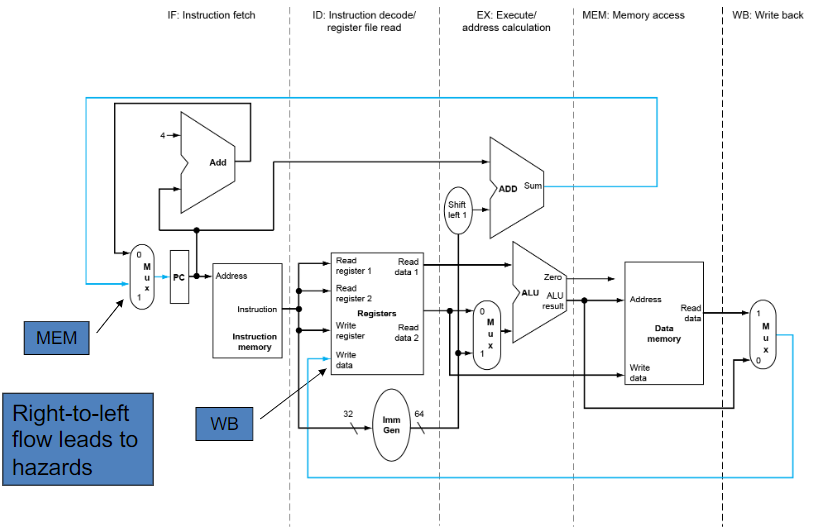
\includegraphics[width=0.479\textwidth]{CO4/RISC-V Pipelined Datapath}
    \caption{RISC-V Pipelined Datapath}
\end{figure}

\subsubsection{Pipeline registers}
To hold information produced in previous cycle,  need registers between stages. 

\begin{figure}[!htb]
    \centering
    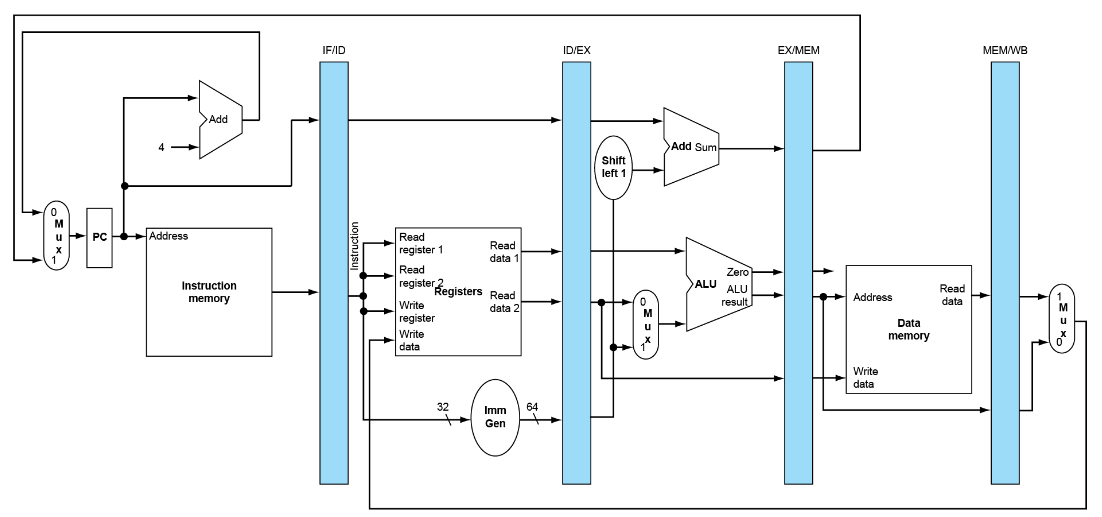
\includegraphics[width=0.479\textwidth]{CO4/Pipeline registers}
    \caption{Pipeline registers}
\end{figure}

\subsubsection{Pipeline Operation}
Cycle-by-cycle flow of instructions through the pipe- lined datapath. 
\begin{itemize}\small
    \item  ``Single-clock-cycle'' pipeline diagram: Shows pipeline usage in a single cycle and Highlight resources used
    \item c.f. “multi-clock-cycle” diagram: Graph of operation over time
\end{itemize}

For Load
\begin{enumerate}\small
    \item IF
    \item ID
    \item EX 
    \item MEM
    \item WB
    \item Corrected Datapath
\end{enumerate}

\paragraph{Multi-Cycle Pipeline Diagram}
Form showing resource usage
\begin{figure}[!htb]
    \centering
    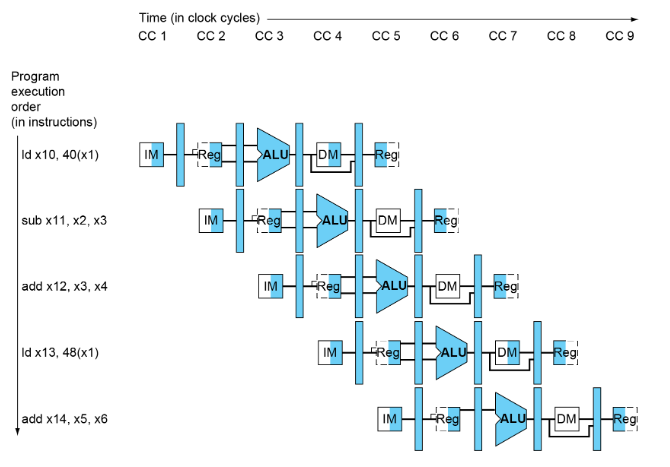
\includegraphics[width=0.47\textwidth]{CO4/Multi-Cycle Pipeline Diagram}
    \caption{Multi-Cycle Pipeline Diagram}
\end{figure}

\paragraph{Single-Cycle Pipeline Diagram}
State of pipeline in a given cycle
\begin{figure}[!htb]
    \centering
    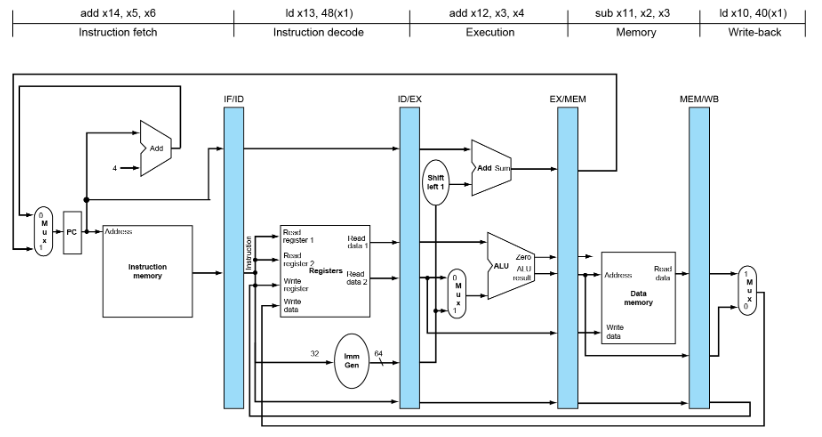
\includegraphics[width=0.449\textwidth]{CO4/Single-Cycle Pipeline Diagram}
    \caption{Single-Cycle Pipeline Diagram}
\end{figure}

\subsubsection{Pipelined Control}
% \begin{figure}[!htb]
%     \centering
%     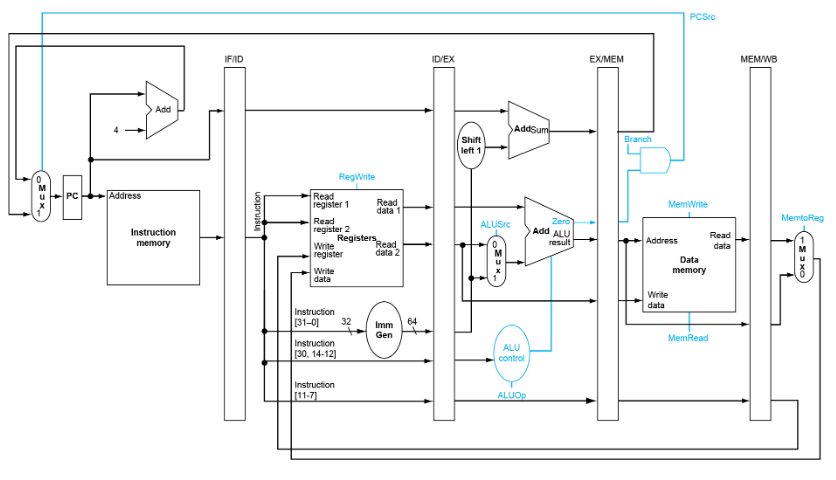
\includegraphics[width=0.449\textwidth]{CO4/Pipelined Control (Simplified)}
%     \caption{Pipelined Control (Simplified)}
% \end{figure}


As in single-cycle implementation, control signals derived from instruction. 

\begin{figure}[!htb]
    \centering
    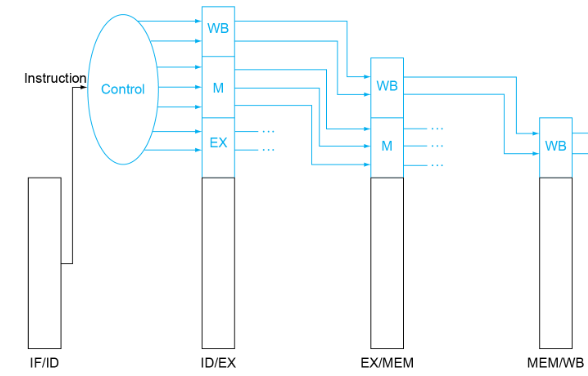
\includegraphics[width=0.309\textwidth]{CO4/control signals}
    \caption{control signals}
\end{figure}

\begin{figure}[!htb]
    \centering
    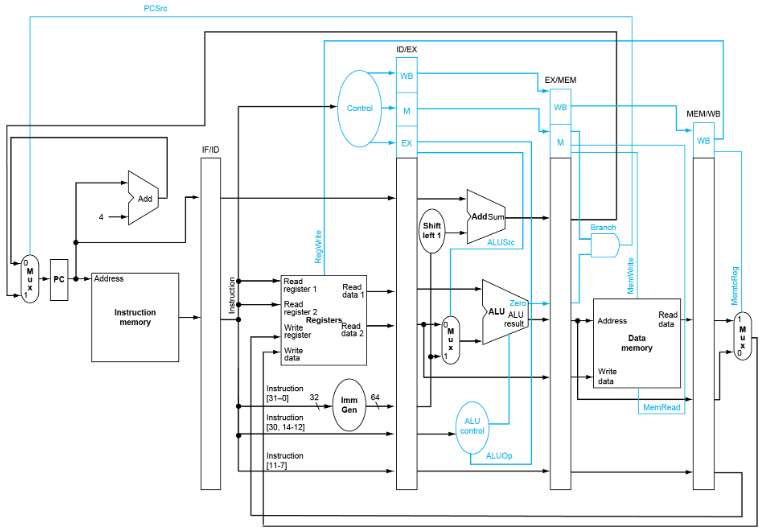
\includegraphics[width=0.479\textwidth]{CO4/Pipelined Control}
    \caption{Pipelined Control}
\end{figure}

\subsection{Data Hazards}
Consider this sequence:
\begin{lstlisting}[language={[x86masm]Assembler}]
sub x2, x1,x3
and x12,x2,x5
or x13,x6,x2
add x14,x2,x2
sd x15,100(x2)
\end{lstlisting}

\subsubsection{Dependencies and Forwarding}
\begin{figure}[!htb]
    \centering
    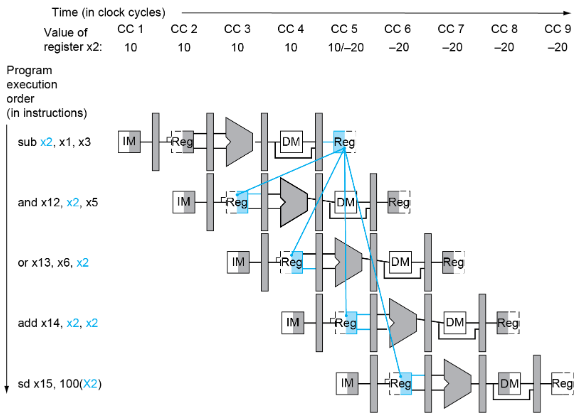
\includegraphics[width=0.479\textwidth]{CO4/Dependencies and Forwarding}
    \caption{Dependencies and Forwarding}
\end{figure}

\paragraph{Detecting the Need to Forward}
Pass register numbers along pipeline.\\ e.g., ID/EX.RegisterRs1 = register number for Rs1 sitting in ID/EX pipeline register. 

ALU operand register numbers in EX stage are given by {ID/EX.RegisterRs1, ID/EX.RegisterRs2}. 

Data hazards when
\begin{align*}
    \left.\begin{array}{c}
        \text{\small EX/MEM.RegisterRd}=\text{\small ID/EX.RegisterRs1}\\
        \text{\small EX/MEM.RegisterRd}=\text{\small ID/EX.RegisterRs2}
    \end{array}\right\} \begin{array}{c}
        \text{\small Fwd from}\\
        \text{\small EX/MEM}\\
        \text{\small pipeline reg}
    \end{array}\\
    \left.\begin{array}{c}
        \text{\small MEM/WB.RegisterRd}=\text{\small ID/EX.RegisterRs1}\\
        \text{\small MEM/WB.RegisterRd}=\text{\small ID/EX.RegisterRs2}
    \end{array}\right\} \begin{array}{c}
        \text{\small Fwd from}\\
        \text{\small MEM/WB}\\
        \text{\small pipeline reg}
    \end{array}
\end{align*}

But only if forwarding instruction will write to a register! EX/MEM.RegWrite, MEM/WB.RegWrite. 

And only if Rd for that instruction is not x0. 
\begin{align*}
    \text{EX/MEM.RegisterRd} &\ne 0\\
    \text{MEM/WB.RegisterRd} &\ne 0
\end{align*}

\begin{figure}[!htb]
    \centering
    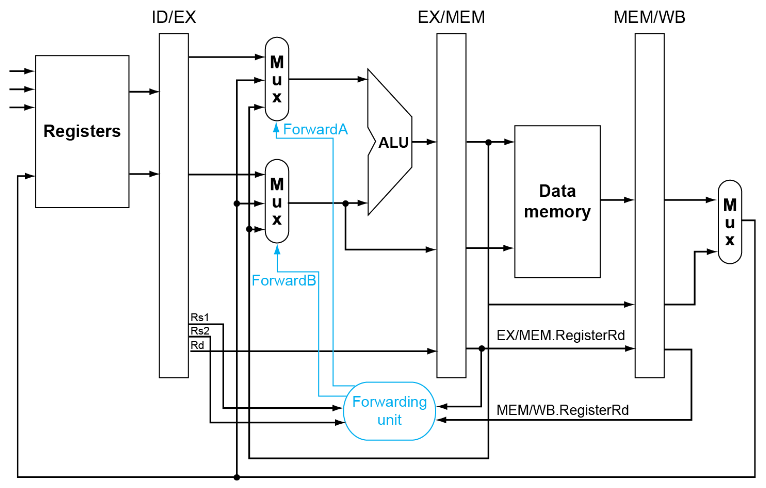
\includegraphics[width=0.47\textwidth]{CO4/Forwarding Paths}
    \caption{Forwarding Paths}
\end{figure}

\begin{table}[!htb]
    \centering
    \caption{Forwarding Conditions}
    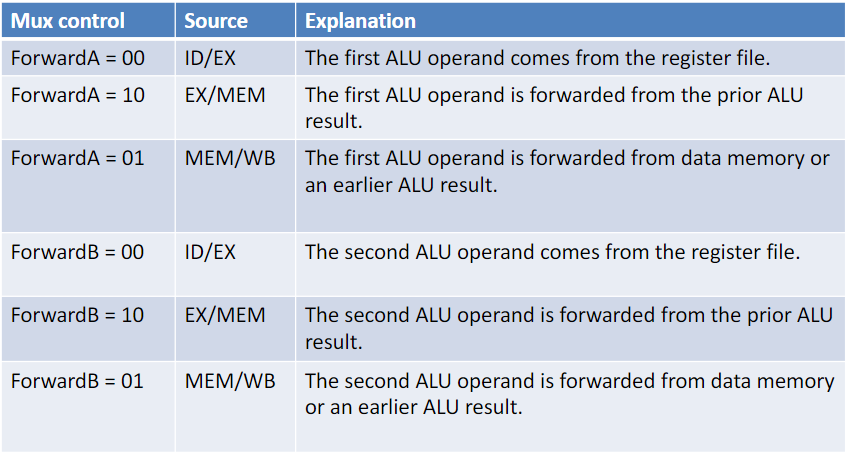
\includegraphics[width=0.479\textwidth]{CO4/Forwarding Conditions}
\end{table}

\subsubsection{Double Data Hazard}
Consider the sequence:
\begin{lstlisting}[language={[x86masm]Assembler}]
add x1,x1,x2
add x1,x1,x3
add x1,x1,x4
\end{lstlisting}

Revise MEM hazard condition, only fwd if EX hazard condition isn't true. 

\paragraph{Revised Forwarding Condition}
MEM hazard

\begin{lstlisting}[language=verilog,morekeywords={set_property,get_ports}, basicstyle=\small]
if (
    MEM/WB.RegWrite
    and (MEM/WB.RegisterRd != 0)
    and not(
        EX/MEM.RegWrite 
        and (EX/MEM.RegisterRd != 0)
        and (EX/MEM.RegisterRd = ID/EX.RegisterRs1)
    )
    and (MEM/WB.RegisterRd = ID/EX.RegisterRs1)
) ForwardA = 01;
\end{lstlisting}
RegisterRs1 is same. 

\begin{figure}[!htb]
    \centering
    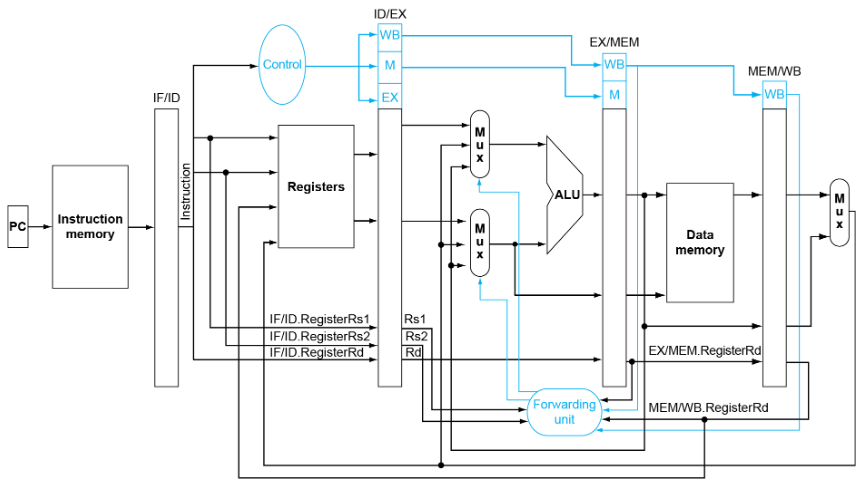
\includegraphics[width=0.47\textwidth]{CO4/Datapath with Forward}
    \caption{Datapath with Forwarding}
\end{figure}

\subsubsection{Load-Use Hazard Detection}
Check when using instruction is decoded in ID stage. 

ALU operand register numbers in ID stage are given by IF/ID.RegisterRs1 or IF/ID.RegisterRs2. 

Load-use hazard when 
\begin{lstlisting}[language=verilog,morekeywords={set_property,get_ports}, basicstyle=\small]
ID/EX.MemRead and (
    (ID/EX.RegisterRd = IF/ID.RegisterRs1) or 
    (ID/EX.RegisterRd = IF/ID.RegisterRs2)
)
\end{lstlisting}

If detected, stall and insert bubble. 

\paragraph{How to Stall the Pipeline}
Force control values in ID/EX register to 0, i.e. EX, MEM and WB do nop (no-operation). 

Prevent update of PC and IF/ID register. 
\begin{enumerate}\small
    \item Using instruction is decoded again
    \item Following instruction is fetched again
    \item 1-cycle stall allows MEM to read data for ld
    \subitem Can subsequently forward to EX stage
\end{enumerate}

\begin{figure}[!htb]
    \centering
    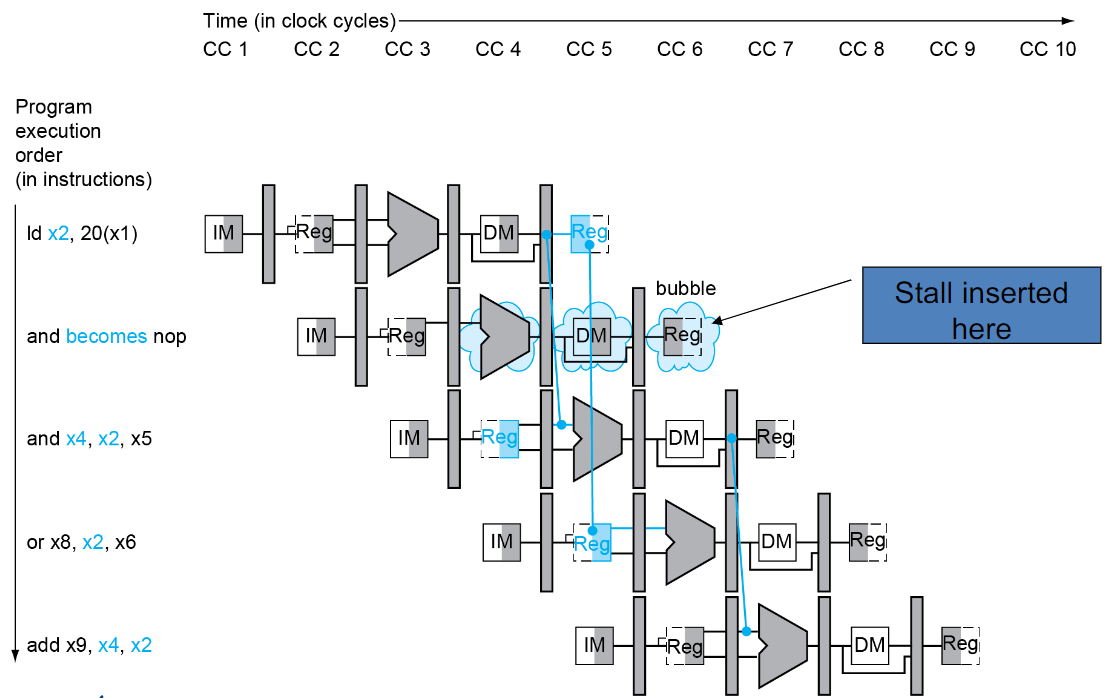
\includegraphics[width=0.439\textwidth]{CO4/Load-Use Data Hazard2}
    \caption{Load-Use Data Hazard}
\end{figure}

\begin{figure}[!htb]
    \centering
    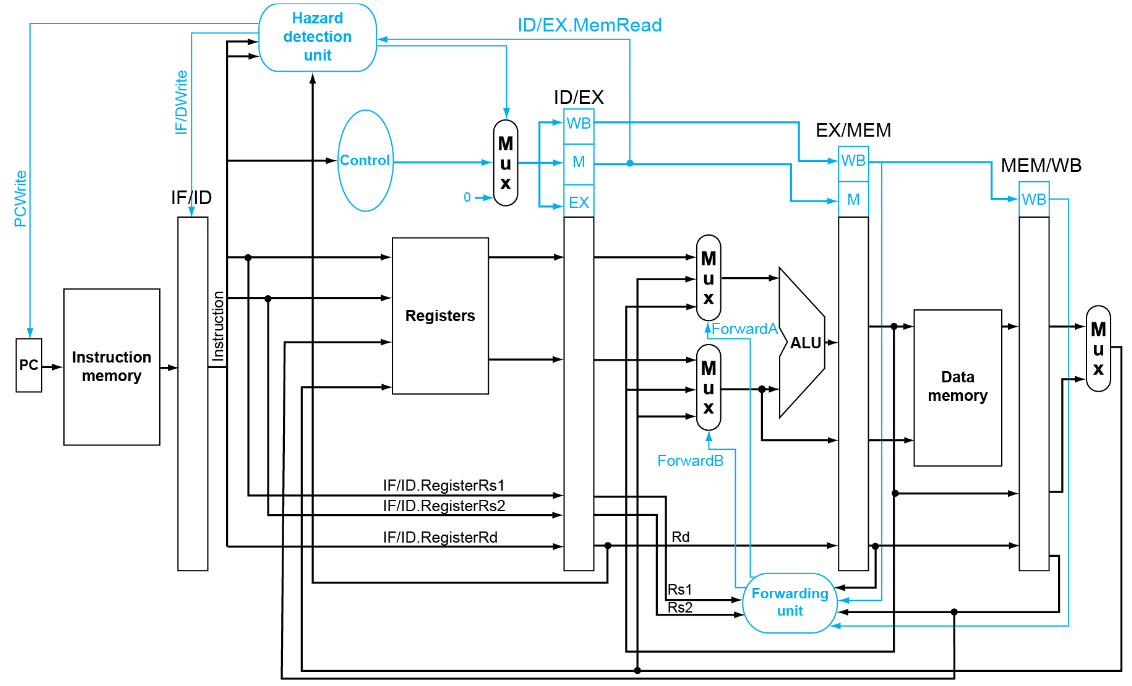
\includegraphics[width=0.439\textwidth]{CO4/Datapath with Hazard Detection}
    \caption{Datapath with Hazard Detection}
\end{figure}


\subsubsection{Stalls and Performance}
Stalls reduce performance, but are required to get correct results. 

Compiler can arrange code to avoid hazards
and stalls.And requires knowledge of the pipeline structure. 

\subsection{Branch Hazards}
If branch outcome determined in MEM, we will lose three instructions

\subsubsection{Reducing Branch Delay}
Move hardware to determine outcome to ID stage. 

Example: branch taken
\begin{lstlisting}[language={[x86masm]Assembler}]
36: sub x10, x4, x8
40: beq x1, x3, 16
44: and x12, x2, x5
48: or  x13, x2, x6
52: add x14, x4, x2
56: sub x15, x6, x7
...
72: ld x4, 50(x7)
\end{lstlisting}
PC-relative branch to 40+16*2=72
% P58-59

\subsubsection{Dynamic Branch Prediction}

Branch prediction buffer (aka branch history table) indexed by recent branch instruction addresses stores outcome (taken/not taken). To execute a branch
\begin{enumerate}\small
    \item Check table, expect the same outcome
    \item Start fetching from fall-through or target
    \item If wrong, flush pipeline and flip prediction
\end{enumerate}

\paragraph{1-Bit Predictor: Shortcoming}
Inner loop branches mispredicted twice. 

\begin{figure}[!htb]
    \centering
    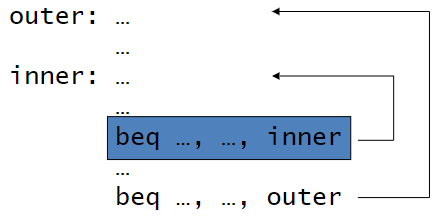
\includegraphics[width=0.309\textwidth]{CO4/Inner loop branches}
    \caption{Inner loop branches}
\end{figure}

Mispredict as taken on last iteration of inner loop. Then mispredict as not taken on first iteration of inner loop next time around. 

\paragraph{2-Bit Predictor}
Only change prediction on two successive mispredictions. 

\begin{figure}[!htb]
    \centering
    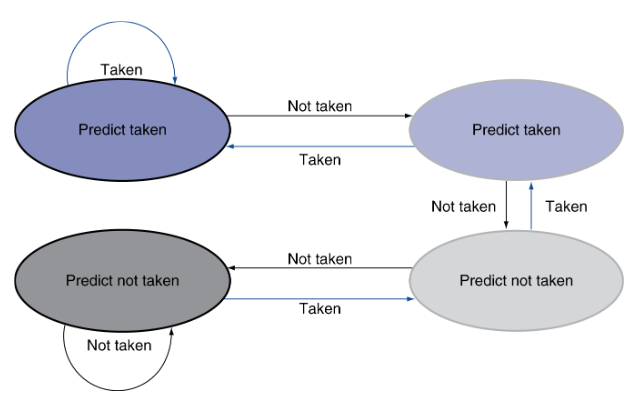
\includegraphics[width=0.439\textwidth]{CO4/2-Bit Predictor}
    \caption{2-Bit Predictor}
\end{figure}

\paragraph{Calculating the Branch Target}
Even with predictor, still need to calculate the target address, 1-cycle penalty for a taken branch. 

Branch target buffer cache of target addresses Indexed by PC when instruction fetched. If hit and instruction is branch predicted taken, can fetch target immediately. 

\subsection{Exceptions and Interrupts}
Exception: Arises within the CPU

Interrupt: From an external I/O controller

\subsubsection{Handling Exceptions}
\begin{enumerate}\small
    \item Save PC of offending (or interrupted) instruction. In RISC-V: Supervisor Exception Program Counter (SEPC)
    \item Save indication of the problem. In RISC-V: Supervisor Exception Cause Register (SCAUSE)
    \item Jump to handler
\end{enumerate}

\paragraph{An Alternate Mechanism}
Vectored Interrupts:\\ Handler address determined by the cause. 

Exception vector address to be added to a vector table base register:
\begin{itemize}\small
    \item Undefined opcode: 00 0100 0000${}_2$
    \item Hardware malfunction: 01 1000 0000${}_2$
    \item $\dots$
\end{itemize}

Instructions either Deal with the interrupt, or Jump to real handler. 

\subsubsection{Handler Actions}
\begin{enumerate}\small
    \item Read cause, and transfer to relevant handler. 
    \item Determine action required
    \item If restartable
    \subitem Take corrective action
    \subitem use SEPC to return to program
    \item Otherwise
    \subitem Terminate program
    \subitem Report error using SEPC, SCAUSE, ...
\end{enumerate}

\subsubsection{Exceptions in a Pipeline}
Exceptions is Another form of control hazard. 

Similar to mispredicted branch, Use much of the same hardware. 

\begin{figure}[!htb]
    \centering
    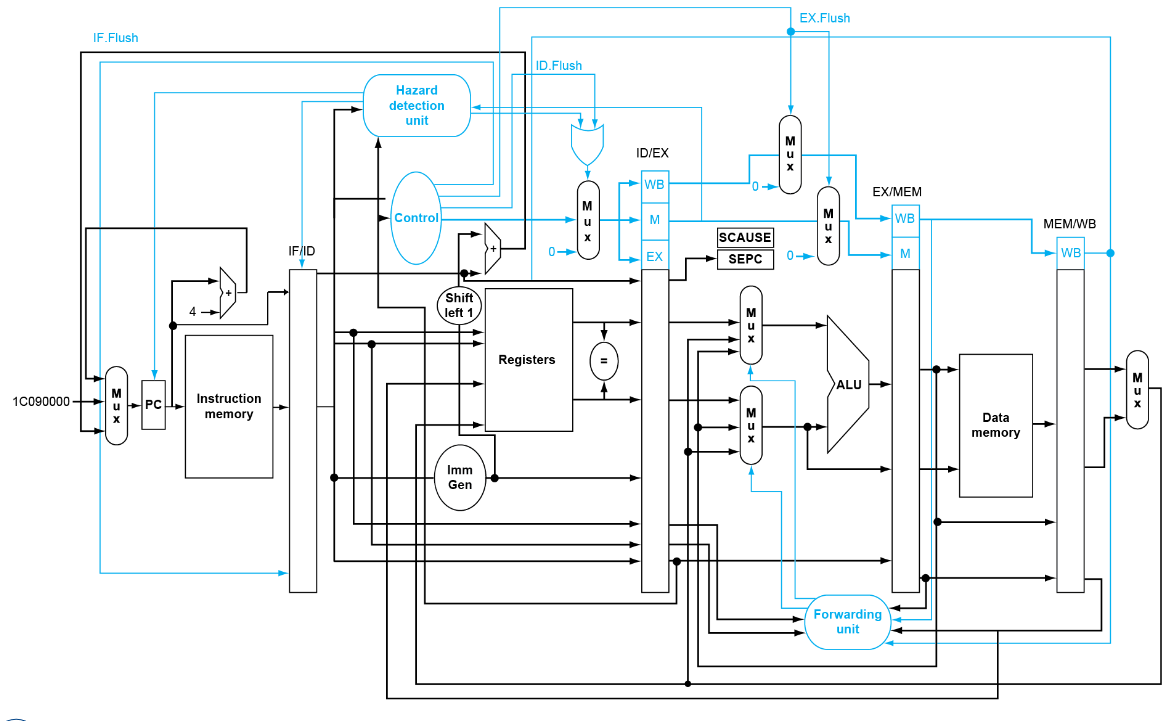
\includegraphics[width=0.479\textwidth]{CO4/Pipeline with Exceptions}
    \caption{Pipeline with Exceptions}
\end{figure}

\paragraph{Exception Properties}
Restartable exceptions:
\begin{itemize}\small
    \item Pipeline can flush the instruction
    \item Handler executes, then returns to the instruction
    \subitem Refetched and executed from scratch
\end{itemize}

PC saved in SEPC register Identifies causing instruction. 

\paragraph{Multiple Exceptions}
Pipelining overlaps multiple instructions could have multiple exceptions at once. 

Simple approach (``Precise'' exceptions): deal with exception from earliest instruction, Flush subsequent instructions. 

In complex pipelines, Multiple instructions issued per cycle, Out-of-order completion, Maintaining precise exceptions is difficult!

\paragraph{Imprecise Exceptions}
Just stop pipeline and save state including exception cause(s). 

Let the handler work out which instruction(s) had exceptions which to complete or flush. May require ``manual'' completion.

Simplifies hardware, but more complex handler software. 

Not feasible for complex multiple-issue out-of-order pipelines. 

\subsection{Instruction-Level Parallelism (ILP)}
Pipelining: executing multiple instructions in parallel. 

To increase ILP:
\begin{enumerate}\small
    \item Deeper pipeline
    \subitem Less work per stage $\Rightarrow$ shorter clock cycle. 
    \item Multiple issue
    \subitem Replicate pipeline stages $\Rightarrow$ multiple pipelines
    \subitem Start multiple instructions per clock cycle
    \subitem CPI $< 1$, so use Instructions Per Cycle (IPC)

    But dependencies reduce this in practice
\end{enumerate}

\subsubsection{Multiple Issue}
\begin{itemize}
    \item Static multiple issue: Compiler groups instructions to be issued together, then packages them into ``issue slots''. It's compiler that detects and avoids hazards. 
    \item Dynamic multiple issue: CPU examines instruction stream and chooses instructions to issue each cycle. Compiler can help by reordering instructions. CPU resolves hazards using advanced techniques at runtime. 
\end{itemize}

\subsubsection{Speculation}
``Guess'' what to do with an instruction
\begin{enumerate}\small
    \item Start operation as soon as possible
    \item Check whether guess was right
    \subitem If so, complete the operation
    \subitem If not, roll-back and do the right thing
\end{enumerate}

Common to static and dynamic multiple issue. 

e.g. 
\begin{itemize}\small
    \item Speculate on branch outcome
    \subitem Roll back if path taken is different. 
    \item Speculate on load
    \subitem  Roll back if location is updated. 
\end{itemize}

\paragraph{Compiler Speculation}
Compiler can reorder instructions, which can include ``fix-up'' instructions to recover from incorrect guess. e.g., move load before branch. 

\paragraph{Hardware Speculation}
Hardware can look ahead for instructions to execute. Buffer results until it determines they are actually needed. Flush buffers on incorrect speculation. 

\paragraph{Speculation and Exceptions}
If exception occurs on a speculatively executed instruction, 
\begin{itemize}\small
    \item Static speculation: Can add ISA support for deferring exceptions. 
    \item Dynamic speculation: Can buffer exceptions until instruction completion (which may not occur). 
\end{itemize}

\subsubsection{Static Multiple Issue}
Compiler groups instructions into ``issue packets'', which is group of instructions that can be issued on a single cycle and determined by pipeline resources required. 

Think of an issue packet as a very long instruction (Very Long Instruction Word (VLIW)), which Specifies multiple concurrent operations .

\paragraph{Scheduling Static Multiple Issue}
Compiler must remove some/all hazards
\begin{enumerate}
    \item Reorder instructions into issue packets
    \item No dependencies with a packet
    \item Possibly some dependencies between packets
    \subitem Varies between ISAs; compiler must know!
    \item Pad with nop if necessary    
\end{enumerate}

\paragraph{RISC-V with Static Dual Issue}
Two-issue packets
\begin{itemize}\small
    \item One ALU/branch instruction
    \item One load/store instruction
    \item 64-bit aligned
    \subitem ALU/branch, then load/store
    \subitem Pad an unused instruction with nop
\end{itemize}

\begin{figure}[!htb]
    \centering
    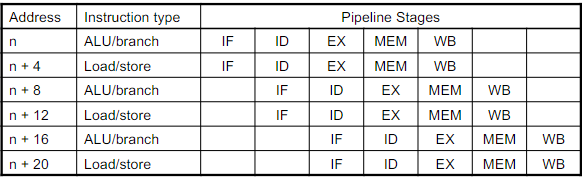
\includegraphics[width=0.479\textwidth]{CO4/RISC-V with Static Dual Issue}
    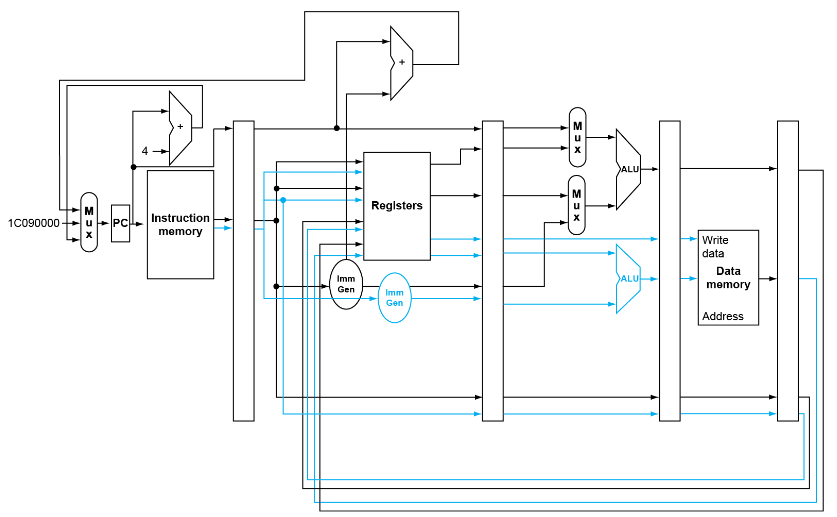
\includegraphics[width=0.479\textwidth]{CO4/RISC-V with Static Dual Issue2}
    \caption{RISC-V with Static Dual Issue}
\end{figure}

\paragraph{Hazards in the Dual-Issue RISC-V}
More instructions executing in parallel. And more aggressive scheduling required
\begin{itemize}\small
    \item EX data hazard
    \subitem Forwarding avoided stalls with single-issue
    \subitem Now can't use ALU result in load/store in same packet, should split into two packets, effectively a stall
    \item Load-use hazard
    \subitem Still one cycle use latency, but now two instructions
\end{itemize}

\paragraph{Scheduling Example}
Schedule this for dual-issue RISC-V
\begin{lstlisting}[language={[x86masm]Assembler}]
Loop:
    ld x31, 0(x20)
    add x31, x31, x21
    sd x31, 0(x20)
    addi x20, x20, -8
    blt ,22, x20, Loop
\end{lstlisting}
\begin{enumerate}\small
    \item x31=array element
    \item add scalar in x21
    \item store result
    \item decrement pointer
    \item branch if x22<x20
\end{enumerate}

\begin{figure}[!htb]
    \centering
    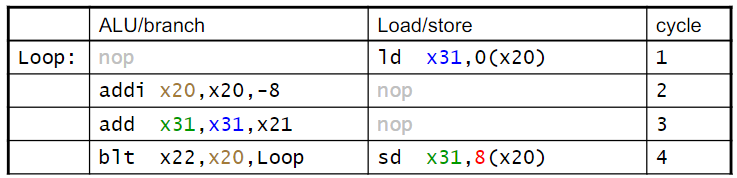
\includegraphics[width=0.42\textwidth]{CO4/Scheduling Example}
    \caption{Scheduling Example}
\end{figure}
IPC = 5/4 = 1.25 (c.f. peak IPC = 2)

\paragraph{Loop Unrolling}
\begin{itemize}\small
    \item Replicate loop body to expose more parallelism
    \subitem which reduces loop-control overhead.
    \item Use different registers per replication
    \subitem called ``register renaming''
    \subitem avoid loop-carried ``anti-dependencies''. 
    \subsubitem store followed by a load of the same register
    \subsubitem Aka ``name dependence'', reuse of a register name
\end{itemize}

\paragraph{Loop Unrolling Example}
\begin{figure}[!htb]
    \centering
    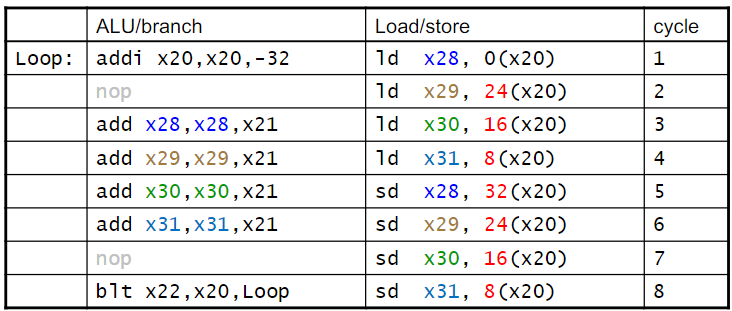
\includegraphics[width=0.42\textwidth]{CO4/Loop Unrolling Example}
    \caption{Loop Unrolling Example}
\end{figure}
IPC = 14/8 = 1.75. Closer to 2, but at cost of registers and code size

\subsubsection{Dynamic Multiple Issue}
CPU decides whether to issue $0, 1, 2, \dots$ each cycle, Avoiding structural and data hazards. 

Avoids the need for compiler scheduling. Though it may still help, code semantics ensured by the CPU


\paragraph{Dynamic Pipeline Scheduling}
Allow the CPU to execute instructions out of
order to avoid stalls, but commit result to registers in order. 

e.g. 
\begin{lstlisting}[language={[x86masm]Assembler}]
    ld x31, 20(x21)
    add x1, x31, x2
    sub x23, x23, x3
    andi x5, x23, 20
\end{lstlisting}
Can start sub while add is waiting for ld

\paragraph{Dynamically Scheduled CPU}
[\ref{Dynamically Scheduled CPU}]
\begin{figure}[!htb]
    \centering
    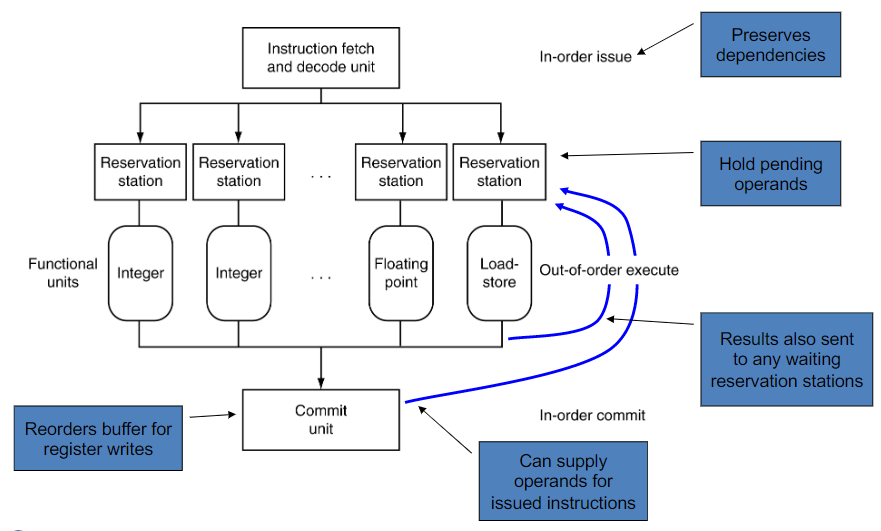
\includegraphics[width=0.42\textwidth]{CO4/Dynamically Scheduled CPU}
    \caption{Dynamically Scheduled CPU}
    \label{Dynamically Scheduled CPU}
\end{figure}


\paragraph{Register Renaming}
Reservation stations and reorder buffer effectively provide register renaming. On instruction issue to reservation station
\begin{itemize}\small 
    \item If operand is available in register file or reorder
    buffer
    \subitem Copied to reservation station
    \subitem No longer required in the register; can be overwritten
    \item  If operand is not yet available
    \subitem It will be provided to the reservation station by a function unit
    \subitem Register update may not be required
\end{itemize}

\paragraph{Speculation}
Predict branch and continue issuing. Don't commit until branch outcome determined. 

Load speculation: Avoid load and cache miss delay
\begin{itemize}\small
    \item Predict the effective address
    \item Predict loaded value
    \item Load before completing outstanding stores
    \item Bypass stored values to load unit
\end{itemize}
Don't commit load until speculation cleared

